%% The first command in your LaTeX source must be the \documentclass command.
%%
%% Options:
%% twocolumn : Two column layout.
%% hf: enable header and footer.
\documentclass[
% twocolumn,
% hf,
]{ceurart}


%%
%% Reviewing packages and definitions
\usepackage[dvipsnames,svgnames]{xcolor} % text color
\usepackage[normalem]{ulem} % wavy underlines
\newcommand{\todo}[1]{\noindent\textcolor{red}{{\bf \{TODO}: #1{\bf \}}}}
\newcommand{\TODO}[1]{\todo{#1}}
\newcommand{\citeneeded}{\textcolor{red}{{\bf [?!]}}}
\newenvironment{draft}{\color{gray}}{\color{black}}
\newcommand\jr[1]{{\color{Red}\textbf{JR}: #1}}

%%
%% One can fix some overfulls
\sloppy

%%
%% Minted listings support 
%% Need pygment <http://pygments.org/> <http://pypi.python.org/pypi/Pygments>
\usepackage[outputdir=build]{minted}
%% auto break lines
\setminted{breaklines=true}

%%
%% end of the preamble, start of the body of the document source.
\begin{document}

%%
%% Rights management information.
%% CC-BY is default license.
\copyrightyear{2022}
\copyrightclause{Copyright for this paper by its authors.
  Use permitted under Creative Commons License Attribution 4.0
  International (CC BY 4.0).}

%%
%% This command is for the conference information
\conference{ISWC'23: International Semantic Web Conference,
  November 06--10, 2023, Athens, Greece}


%%
%% The "title" command
\title{Bringing IDE Support to JSON-LD with the Language Server Protocol}

% \tnotemark[1]
% \tnotetext[1]{You can use this document as the template for preparing your
%   publication. We recommend using the latest version of the ceurart style.}

%%
%% The "author" command and its associated commands are used to define
%% the authors and their affiliations.
\author[1]{Author 1}[%
orcid=0000-0000-0000-0000,
]
\author[1]{Author 2}[%
orcid=0000-0000-0000-0000,
]
\author[1]{Author 3}[%
orcid=0000-0000-0000-0000,
]
\address[1]{Some place on the world}


%%
%% The abstract is a short summary of the work to be presented in the
%% article.
\begin{abstract}
  JSON-LD is a popular data format used to describe and share semantic data on the web.
  However, creating and editing JSON-LD documents can be a challenging task, especially when dealing with complex contexts that include many properties.
  The existing JSON editing functionality may not suffice for developers, and a JSON-LD editor could greatly enhance their experience.
  In this paper, we introduce a JSON-LD Language Server Protocol (LSP) that empowers text editors compatible with the LSP protocol (e.g., Visual Studio Code and NeoVim) with IDE functionality, including autocompletion suggestions based on the defined context, semantic highlighting and renaming identifiers inside the document.
  We believe that a JSON-LD LSP will enhance developer ergonomics and promote its adoption.
  Moreover, we see high potential for additional features that can be added such as hovering, go-to-definition and code actions like flattening or structuring of JSON-LD documents.
\end{abstract}

%%
%% Keywords. The author(s) should pick words that accurately describe
%% the work being presented. Separate the keywords with commas.
\begin{keywords}
  Linked Data \sep 
  JSON-LD \sep
  Language Server
\end{keywords}

%%
%% This command processes the author and affiliation and title
%% information and builds the first part of the formatted document.
\maketitle

\section{Introduction}

JSON-LD is a data serialization format that is used to describe semi-structured data on the web \cite{JSON-LD-W3C}.
It adds semantic information to JSON, among others with the \textit{@context} property, pointing to a JSON-LD context.
This context specifies how to map properties to predicates, called aliases.

With its increasing popularity, contexts in JSON-LD also increase in complexity.
For example, the Flemish (Belgium) OSLO initiative is working to achieve interoperability by building semantic standards for different stakeholders such as government, industry and academia \footnote{\href{https://www.vlaanderen.be/digitaal-vlaanderen/onze-oplossingen/oslo}{OSLO} - Open Standaarden voor Linkende Organisaties}.
They focus on standardizing JSON-LD context files for their vocabularies and application profiles. 
An example is \href{https://data.vlaanderen.be/doc/applicatieprofiel/vlaamse-codex/}{the Flemish codex application profile}, the context defined for this profile enables the usage of Dutch JSON objects to be Linked Data.

Another example where JSON-LD contexts are extensively used is the semantic dependency injection framework ComponentsJs \cite{CJS}. 
ComponentsJs allows Javascript packages to define JSON-LD contexts that describe the package, these contexts are then used to configure an instance of a program.

Creating new JSON-LD documents is a difficult task, to know the defined aliases the developer has to scrupulously explore the context and remember the defined names, 
accidental typos can result in broken linked data and to the best of our knowledge, there are no tools in existence that could assist in preventing this issue.
We show that using a language server for JSON-LD helps alleviate this problem and can also bring better developer ergonomics for experienced and new semantic web developers.

Similar efforts have been made before, but never for JSON-LD. 
For example, the Yasgui editor\footnote{\href{https://triply.cc/docs/yasgui/}{Yasgui} - SPARQL editor}, a popular SPARQL human query interface, provides autocompletion based on the LOV API \cite{LOV}. 
Plugins can add autocompletion based on domain knowledge. 
These capabilities are built into the deployed editor and can only be used with Yasgui.
Stardog created open-source LSPs for turtle, TRIG, SPARQL, and more, however, they focus only on correct syntax and keyword auto-completion \cite{stardog}. 

We make our demo JSON-LD LSP and installation instructions to be used with LSP capable editors available at Github (MIT).


\section{Language Server Protocol}

The Language Server Protocol (LSP) is a JSON RPC protocol developed by Microsoft to simplify the process of integrating language-specific logic into an editor \footnote{\href{https://microsoft.github.io/language-server-protocol/}{LSP} - Language Server Protocol}. 
Prior to LSP, editors had to implement each programming language they wanted to support individually, resulting in an \(O(n*m)\) complexity where n is the number of editors and m is the number of programming languages.
With LSP, editor and language-specific logic only needs to be implemented once, resulting in a much simpler \(O(n+m)\) complexity \cite{LSP-Multi}.
LSP only concerns itself with the source files of the program and doesn't involve building, running, or debugging.
This is in contrast to the Build Server Protocol \footnote{\href{https://github.com/build-server-protocol/build-server-protocol}{BSP} - Builder Server Protocol}.

Next we discuss the main features a LSP provides to an editor and discuss how these features may be useful in the context of JSON-LD.

\begin{itemize}
  \item \textbf{Autocompletion} enables the developer to type less and thus make less mistakes. It also shows the developer more options so not all aliases have to be known by heart.
  \item \textbf{Diagnostics} represent errors in the file, this goes from syntax errors to warnings that inform the developer that for example a property is not defined in the current context.
  \item \textbf{Semantic Highlighting} differs from syntax highlighting. The syntax of JSON is very easy, but semantic highlighting shows used keywords and variable identifiers etc. \jr{Maybe an example here?}
  \item \textbf{Code actions} are general actions. For JSON-LD these can be e.g., flattening, compacting or expanding the structure. General actions like renaming and formatting could also supported.
  \item \textbf{Hover} can show additional information about properties. By using the power of linked data, the IDE can dereference the property and look for some description of the used property.
\end{itemize}

The protocol allows for partial implementations, in the next section we show a demo that implements some of these features and yet, already shows to significantly improve JSON-LD editing experience.

\section{Demo}

Our demo presents an implementation of a JSON-LD Language Server Protocol (LSP), developed using the Rust programming language and based on a basic LSP implementation \footnote{\href{https://crates.io/crates/tower-lsp}{Tower LSP} - Crate by Eyal Kalderon}.
To extract predicate mappings from the context, we rely on the JSON-LD crate \footnote{\href{https://crates.io/crates/json-ld}{JSON-LD} - Crate by Timothée Haudebourg}.
The full source code and installation instructions can be found on GitHub (MIT).
This LSP is available on the web, as a vscode extension and as a NeoVim LSP. Documentation is also available on the website. 

The demo implementation supports autocompletion, diagnostics and semantic highlighting and renaming (each with their own caveats). 
Autocompletion only supports simple and explicit aliases extracted from the context. 
It should be possible to write \textit{foaf:} and get autocompletion for all defined predicates in the \textit{foaf} namespace, but this is not yet supported.
Diagnostics only gives syntax diagnostics, however the demo does not warm developers if an undefined predicate is used.
Semantic highlighting works as expected and shows keywords and identifiers in different colors.


\begin{figure}
\centering
\makebox[\textwidth][c]{
    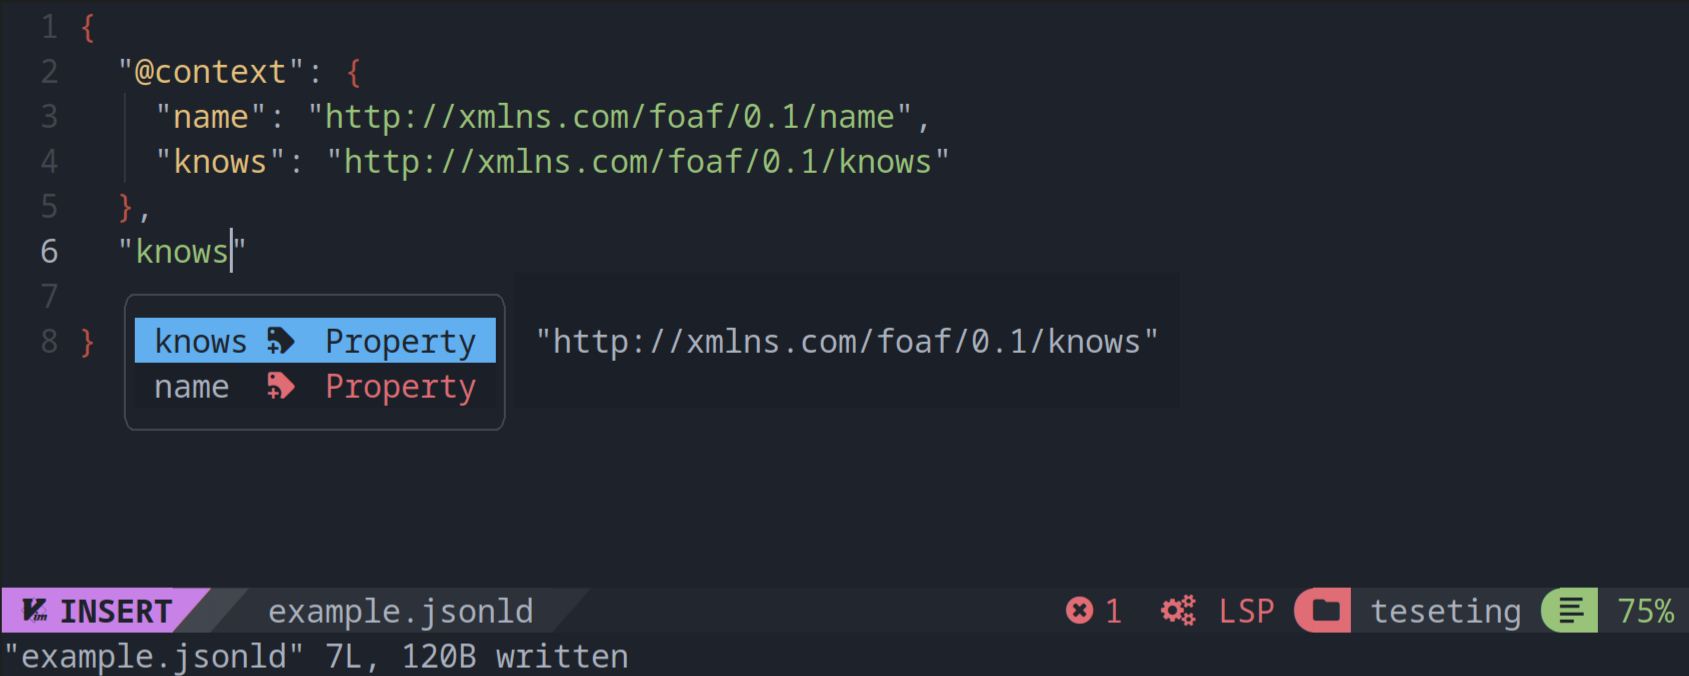
\includegraphics[width=.5\linewidth]{./fig/completion.png}
    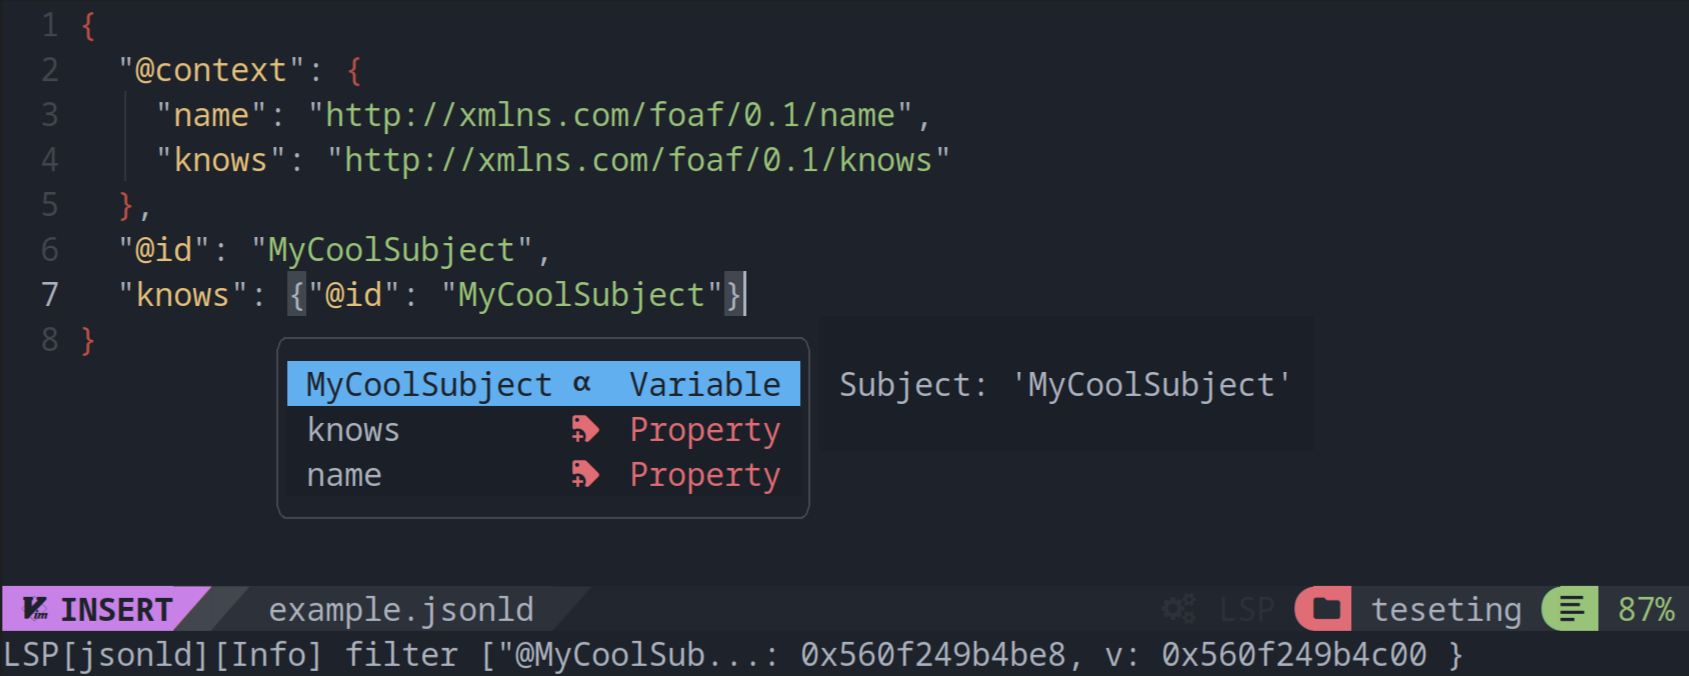
\includegraphics[width=.5\linewidth]{./fig/completion-id.png}
}
\caption{Screenshots showing completion functionality in NeoVim: left a list with all completion options, right a list containing the defined subject.}
\label{fig:complete}
\end{figure}


One of the key features of our LSP is code autocompletion based on the defined context. It extracts aliases from the inlined context, local contexts, and contexts hosted on the web. However, it currently does not take into account special context attributes such as context overloading or scoped contexts \cite{JSON-LD-W3C}. Figure \ref{fig:complete}, shoes this in action. The context defines two aliases, "name" and "knows". When the completion event is triggered, the user can choose between these aliases and the editor will complete the chosen alias. Defined subjects can be completed when writing \textit{@}, but will expand to more involved objects.

\begin{figure}
\centering
\makebox[\textwidth][c]{
    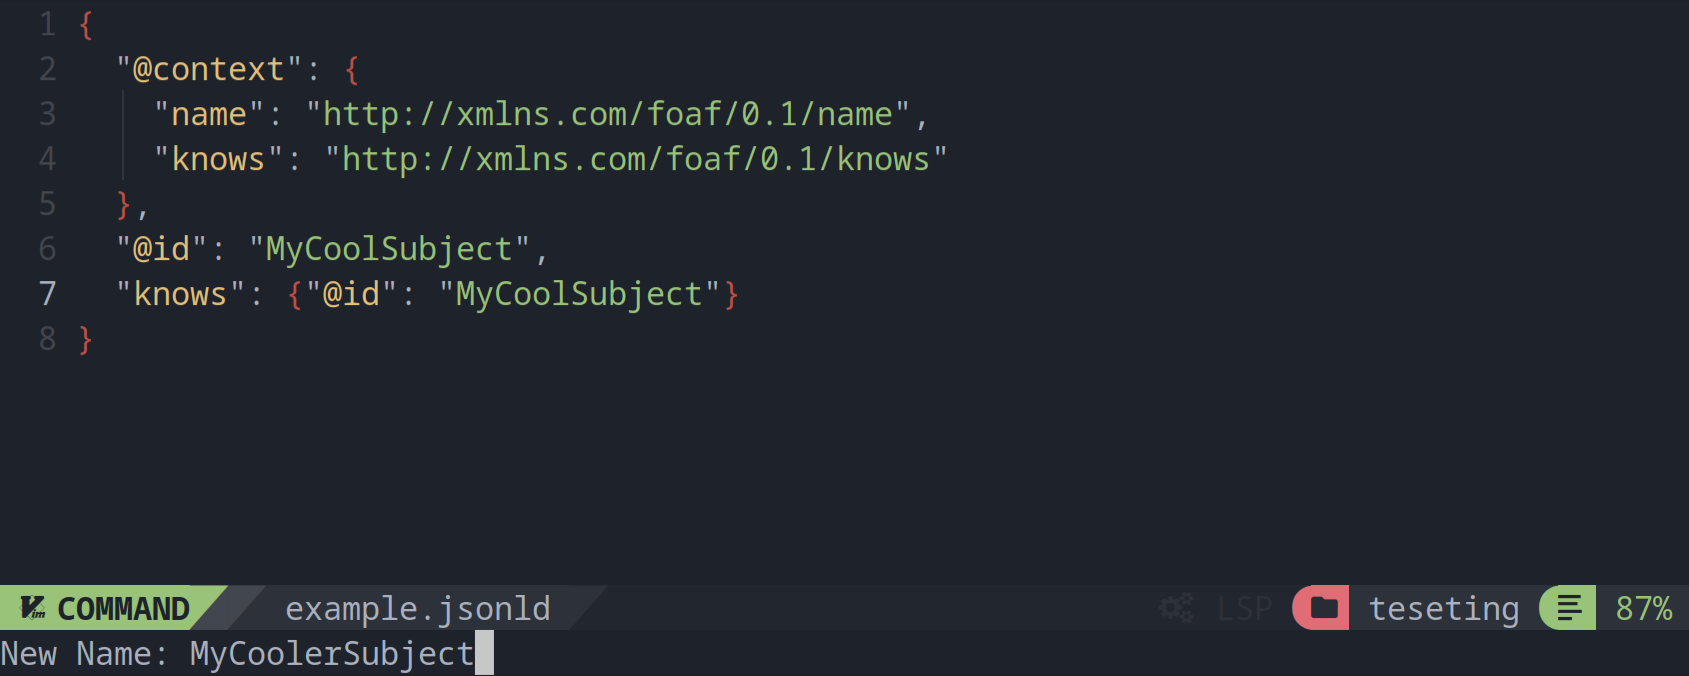
\includegraphics[width=.5\linewidth]{./fig/rename-1-small.png}
    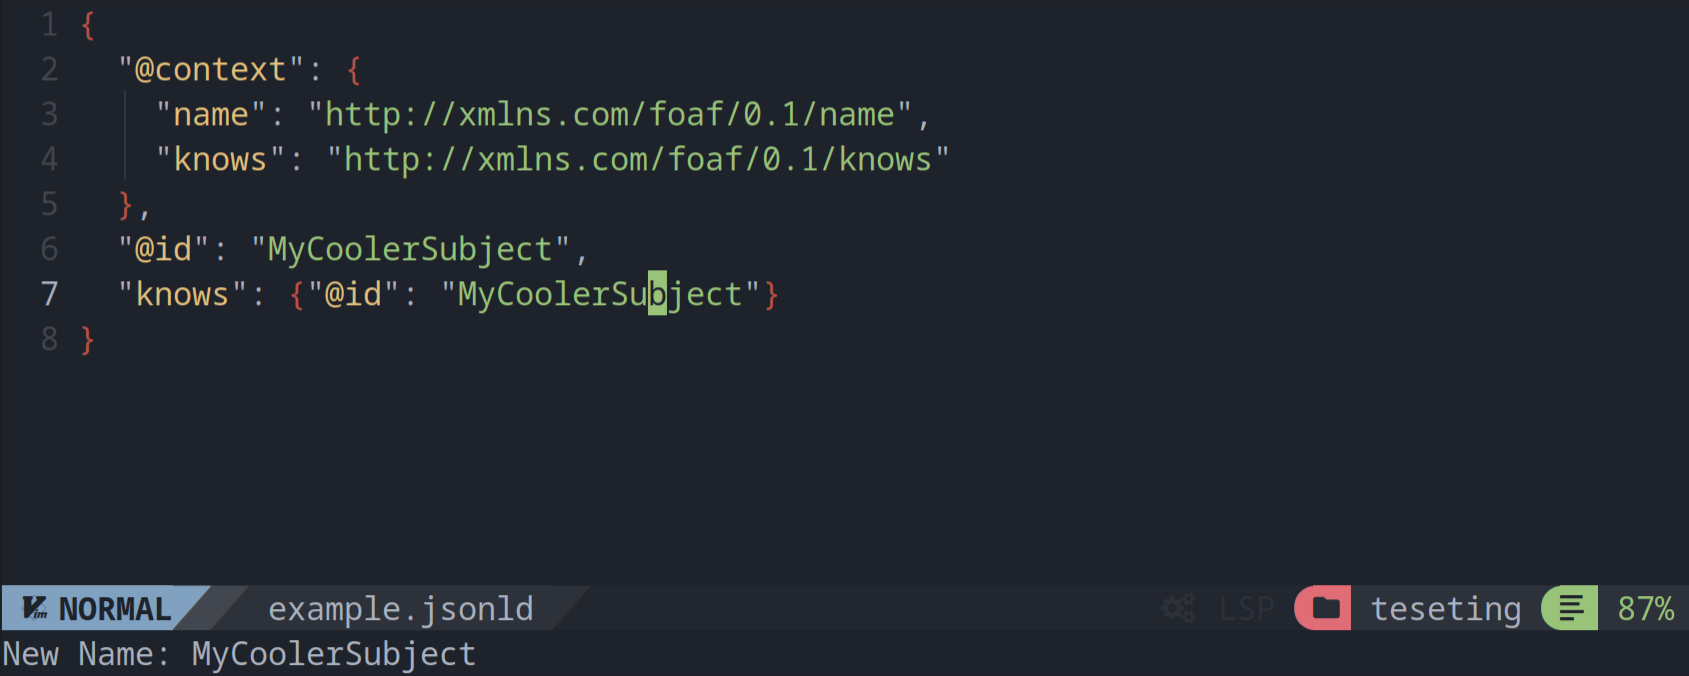
\includegraphics[width=.5\linewidth]{./fig/rename-2-small.png}
}
\caption{Screenshots showing renaming functionality in NeoVim: left NeoVim asks for the new name, right the subject is renamed.}
\label{fig:rename}
\end{figure}

Additionally, our LSP implementation supports renaming subjects. This is shown in Figure \ref{fig:rename}. The user is asked for the new name and the LSP server will respond with the required text changes that change all matching subjects to the new name.



\section{Conclusion}

This demonstration merely scratches the surface of the vast capabilities of a JSON-LD LSP.
By leveraging fully-interpreted contexts, the LSP can provide more contextually-relevant suggestions, taking into account context overloading and scoped contexts. 
Additionally, the LSP's functionality can be expanded to include the interpretation of referenced vocabularies, allowing completion for compacted predicates, like \textit{foaf:knows}.
Despite its current limitations, the LSP already enhances the developer experience by facilitating the creation and editing of JSON-LD documents.


%%
%% Define the bibliography file to be used
\jr{There is an issue in reference [3]}
\bibliography{bibliography}


\end{document}

%%
%% End of file

